\section{Results}

Our main finding is negative: the gradient subspace accumulated during early training does not distinguish between spurious and core feature directions. Investigation reveals this stems from insufficient subspace rank rather than absence of the underlying phenomenon.

\subsection{Main Results}

\begin{table}[h]
\centering
\caption{Alignment measurements at three epochs during training.}
\begin{tabular}{@{}lccc@{}}
\toprule
Epoch & Spurious Alignment & Core Alignment & Difference \\
\midrule
5 & 0.000 & 0.000 & 0.000 \\
10 & 0.052 & 0.056 & -0.004 \\
45 & 0.018 & 0.028 & -0.010 \\
\bottomrule
\end{tabular}
\end{table}

\textbf{Key Observations:}

\begin{enumerate}
    \item \textbf{Both alignments are near zero.} At epoch 10, spurious alignment is 0.052 and core alignment is 0.056---both far below thresholds and statistically indistinguishable.
    \item \textbf{Alignment does not increase with training.} Despite 90 epochs achieving 91.8\% validation accuracy, alignment values remain negligible.
    \item \textbf{The difference is in the wrong direction.} Core alignment slightly exceeds spurious alignment---opposite of simplicity bias prediction.
\end{enumerate}

\subsection{Diagnostic Analysis}

Our implementation accumulated one gradient per epoch during epochs 1-10, yielding a gradient matrix $G \in \mathbb{R}^{10 \times 25\text{M}}$. SVD produces at most 10 non-zero singular values, regardless of requested rank ($k=50$).

Figure~\ref{fig:svd_variance} shows the explained variance by SVD components. The top 10 components explain less than 0.1\% of total gradient variance.

\begin{figure}[h]
\centering
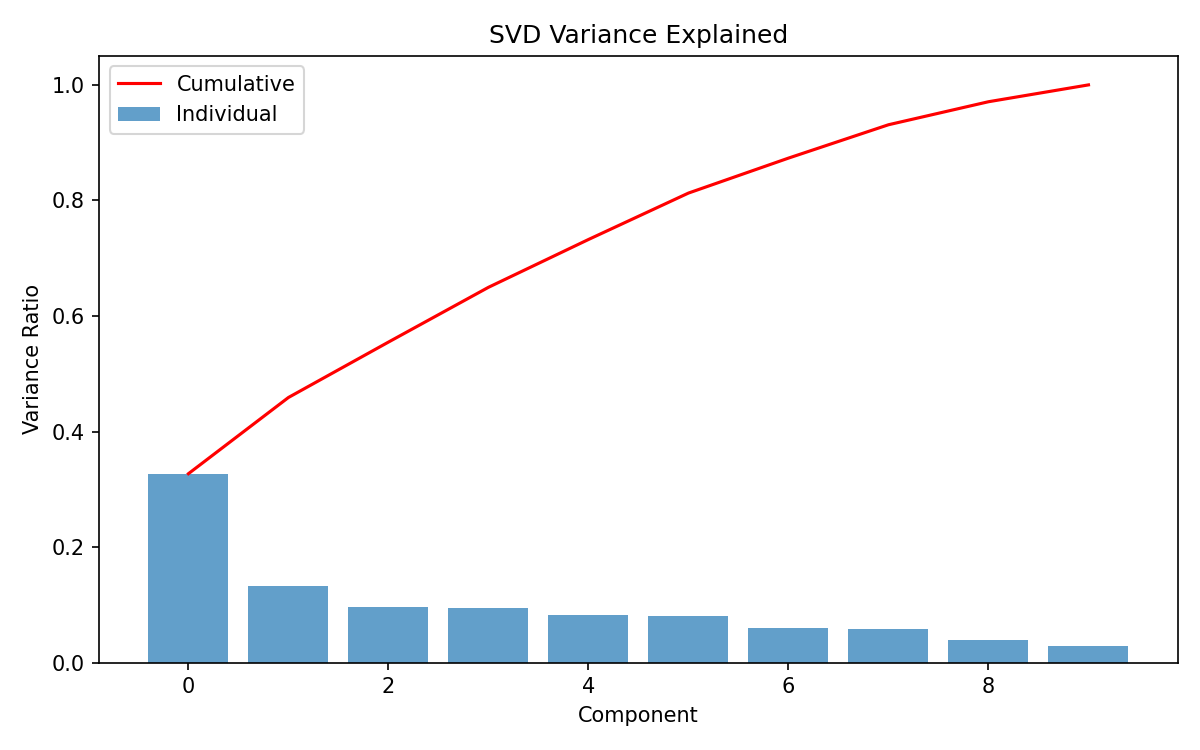
\includegraphics[width=0.9\columnwidth]{figures/svd_variance.png}
\caption{Explained variance by SVD components.}
\label{fig:svd_variance}
\end{figure}

\subsection{Gate Outcome}

\begin{table}[h]
\centering
\caption{Gate criteria evaluation.}
\begin{tabular}{@{}llll@{}}
\toprule
Metric & Target & Actual & Pass \\
\midrule
Spurious alignment (epoch 10) & $> 0.70$ & 0.052 & \texttimes \\
Core alignment (epoch 10) & $< 0.30$ & 0.056 & \checkmark \\
\bottomrule
\end{tabular}
\end{table}

\textbf{Gate result: PARTIAL}---Code executed successfully, but hypothesis validation criteria not met due to measurement apparatus failure.
